\documentclass[a4paper]{article}

\usepackage[pagebackref=false,colorlinks,urlcolor = blue,linkcolor=blue,citecolor=blue]{hyperref}

\usepackage{indentfirst}
\usepackage{amsmath,amsfonts,amssymb,amsthm}
\usepackage{geometry}
\usepackage{enumitem}
\usepackage{amsmath}
\usepackage[usenames,dvipsnames]{color,xcolor}
\definecolor{mygreen}{RGB}{28,172,0} % color values Red, Green, Blue
\definecolor{mylilas}{RGB}{170,55,241}
\usepackage{listings}
\usepackage{hyperref}
\hypersetup{linkcolor=blue}
\usepackage{graphicx}
\usepackage{emptypage}
\usepackage{afterpage}
\usepackage{titlesec}
\usepackage{wrapfig}
\usepackage{tikz}
\usetikzlibrary{arrows,decorations.markings}

\titleformat{\section}
{\normalfont\fontsize{20}{20}\bfseries}{\thesection}{1em}{}

\titleformat{\subsection}
{\normalfont\fontsize{15}{20}\bfseries}{\thesubsection}{1em}{}

\titleformat{\subsubsection}
{\normalfont\fontsize{12}{20}\bfseries}{\thesubsubsection}{1em}{}

\usepackage{pdfpages}
\usepackage{tikz}
\usepackage[american]{circuitikz}
\renewcommand{\baselinestretch}{1.2} 
\lstset{language=Matlab,%
	%basicstyle=\color{red},
	breaklines=true,%
	morekeywords={matlab2tikz},
	keywordstyle=\color{blue},%
	morekeywords=[2]{1}, keywordstyle=[2]{\color{black}},
	identifierstyle=\color{black},%
	stringstyle=\color{mylilas},
	commentstyle=\color{mygreen},%
	showstringspaces=false,%without this there will be a symbol in the places where there is a space
	numbers=left,%
	numberstyle={\tiny \color{black}},% size of the numbers
	numbersep=9pt, % this defines how far the numbers are from the text
	emph=[1]{for,end,break},emphstyle=[1]\color{blue}, %some words to emphasise
	%emph=[2]{word1,word2}, emphstyle=[2]{style},    
}

\geometry{
	a4paper,
	total={170mm,257mm},
	left=20mm,
	top=20mm,
}

\usepackage{xcolor}
\usepackage{listings}

\definecolor{mGreen}{rgb}{0,0.6,0}
\definecolor{mGray}{rgb}{0.5,0.5,0.5}
\definecolor{mPurple}{rgb}{0.58,0,0.82}
\definecolor{backgroundColour}{rgb}{0.95,0.95,0.92}


\lstdefinestyle{JavaStyle}{
	backgroundcolor=\color{backgroundColour},   
	commentstyle=\color{mGreen},
	keywordstyle=\color{magenta},
	numberstyle=\tiny\color{mGray},
	stringstyle=\color{mPurple},
	  basicstyle=\ttfamily\small,
	breakatwhitespace=false,         
	breaklines=true,                 
	captionpos=b,                    
	keepspaces=true,                 
	numbers=left,                    
	numbersep=5pt,                  
	showspaces=false,                
	showstringspaces=false,
	showtabs=false,                  
	tabsize=2,
	language=java
}



\usepackage{fancyhdr}
\pagestyle{fancy}
\fancyhf{}
\rhead{\textbf{Phase \#2}}
\lhead{\textbf{Advanced Programming Project}}
\cfoot{(\space \space \space \space \textbf{\thepage}  \space \space \space)}
\renewcommand{\headrulewidth}{1pt}
\renewcommand{\footrulewidth}{1pt}
\setlength{\parindent}{0ex}
\setlength{\parskip}{0ex}


%\usepackage{xepersian}
%\setlatintextfont[Scale=1]{Times New Roman}
%\settextfont{XB Niloofar}
%\setdigitfont{XB Niloofar}
%\DefaultMathsDigits 
%\makeatletter
%\bidi@patchcmd{\@Abjad}{آ}{الف}
%{\typeout{Succeeded in changing `آ` into `الف`}}
%{\typeout{Failed in changing `آ` into `الف`}}
%\makeatother
%\PersianAlphs

\DeclareMathOperator*{\epi}{\mathbf{epi}\space} 
\DeclareMathOperator*{\hypo}{\mathbf{hypo}\space} 
\DeclareMathOperator*{\dom}{\mathbf{dom}\space} 
\DeclareMathOperator*{\intt}{\mathbf{int}\space} 
\DeclareMathOperator*{\diag}{\mathbf{diag}\space} 
\DeclareMathOperator*{\minmz}{\mathrm{minimize}\:} 
\DeclareMathOperator*{\maxmz}{\mathrm{maximize}\:} 
\DeclareMathOperator*{\tr}{\mathrm{trace}} 
\DeclareMathOperator*{\st}{\mathrm{subject\:to}\:} 

\begin{document}
	
\begin{titlepage}
	
	\begin{center}
		\textbf{
			In The Name Of God\\
		}
		\vspace{2cm}
		
\includegraphics[scale=0.25]{logo.png}\\
		\vspace{0.5cm}
		\begin{Large}
			\textbf{
				Sharif University of Technology\\
				\vspace{0.5cm}
				Computer Science Department\\
			}
		\end{Large}
		\vspace{2.5cm}
		\begin{huge}
			\textbf{
				Advanced Programming Project\\
				 Phase 2\\
				\vspace{1cm}
				Hearthstone\\
			}
		\end{huge}
		\vspace{1.5cm}
		\begin{Large}
			\textbf{
				\\
				\vspace{1cm}
				Amirhossein Afsharrad\\
				\vspace{0.5cm}
				95101077\\
				\vspace{2cm}
				\today
			}
		\end{Large}
		
	\end{center}
	
	\thispagestyle{empty}
\end{titlepage}	

\large
\tableofcontents
\clearpage
\section{Introduction}
In this document we briefly explain the important points of the implementation of Hearthstone project's second phase. The goal for this phase is to implement the graphical interface of the game, so the game logic has been through slight changes compared to the previous phase; and the game is not ready to be completely played yet. You may find all packages and classes attached to this report, or you can check them using the following link on GitHub:
\begin{center}
	\url{https://github.com/AmirAfsharrad/Hearthstone}
\end{center}
The java version of this project is java11 and it has been built using \textit{Gradle}. Apart from java standard packages, only the two following dependencies have been added to the \texttt{build.gradle} file for the \texttt{gson} and \texttt{json} respective packages:
\begin{itemize}
	\item \texttt{compile 'com.googlecode.json-simple:json-simple:1.1.1'}
	\item \texttt{compile group: 'com.google.code.gson', name: 'gson', version: '2.8.5'}
\end{itemize}

\clearpage
\section{What has changed since phase 1?}
Apart from full implementation of the graphical user interface, the game logic has only had small changes. The most important item to be mentioned is the change in the identity of a \textit{deck}, which used to an array list for each hero; but in this phase has turned into an independent object who may have a hero and a name. To be more specific, the class \texttt{Deck} has been declared containing a name, a hero, and an array list of cards. Each user may have as many decks as he wishes, and can edit all the attributes of a deck. Having to save user's all decks also resulted in some modifications of the code responsible for saving and loading the game.\\

Another change to be mentioned is the addition of more places to the game. In phase 1 we had designed the abstract class \texttt{Place} which was an abstraction of all places a user can visit throughout the game. These places included \texttt{SignInOrSignUp}, \texttt{MainMenu}, \texttt{Store} and \texttt{Collections}. For this phase we have add more places: \texttt{Playground}, \texttt{Status}, and \texttt{InfoPassive}.\\

Apart from the two points just mentioned, there are no major differences in the game logic compared to the previous phase.

\clearpage
\section{The GUI General Structure}
As mentioned before, the major goad to this phase was to implement the graphical user interface of the game. To achieve this goal, we have several new classes, the most important of which is the \textit{Mainframe}. \textit{The Mainframe acts as a controller and an intermediary link between the logic and the GUI}. To be more specific, no graphical panel makes a change in the game logic, unless making in through the mainframe. This makes the logic and the GUI quite separate, which is a key feature in the program's structure.\\

The next three sections are dedicated to a brief review of the five packages designed for the GUI. After that, we also review the resources we have used for this phase of the project. Before starting that, to gain a better understanding fo the general structure, note that the main frame is managed be the swing's \texttt{CardLayout} layout manager, and each place of the game (which has a panel) is a card in this card layout. As a result, the game controller brings the appropriate card to the front whenever an event happens in the game.


\clearpage
\section{Package \texttt{GamePanels}}
This package is the most important package responsible for the game graphics. Inside that, there exists an abstract class called \texttt{GamePanel}, which is the abstraction of a panel existing inside a game. To be more specific about the panels, note that there is a one to one correspondence between the game places and the game panels. For each place, we have designed a panel to let the user what he can do when he is inside that place. As a result, there exist seven classes in this package who extend the \texttt{GamePanel} abstract class.\\

While designing these panels, we have tried to make the most use of swing's layouts, and we also have used the absolute positioning method whenever needed. We shall review these panels briefly in the following subsections.
\subsection{\texttt{LoginPanel}}
This panel is responsible for taking the username and password as the input, and to log in for a previously-registered user, or to create a new account for a new one. Figure \ref{loginPanel} shows this panel.

\begin{figure}[h!]
	\centering
	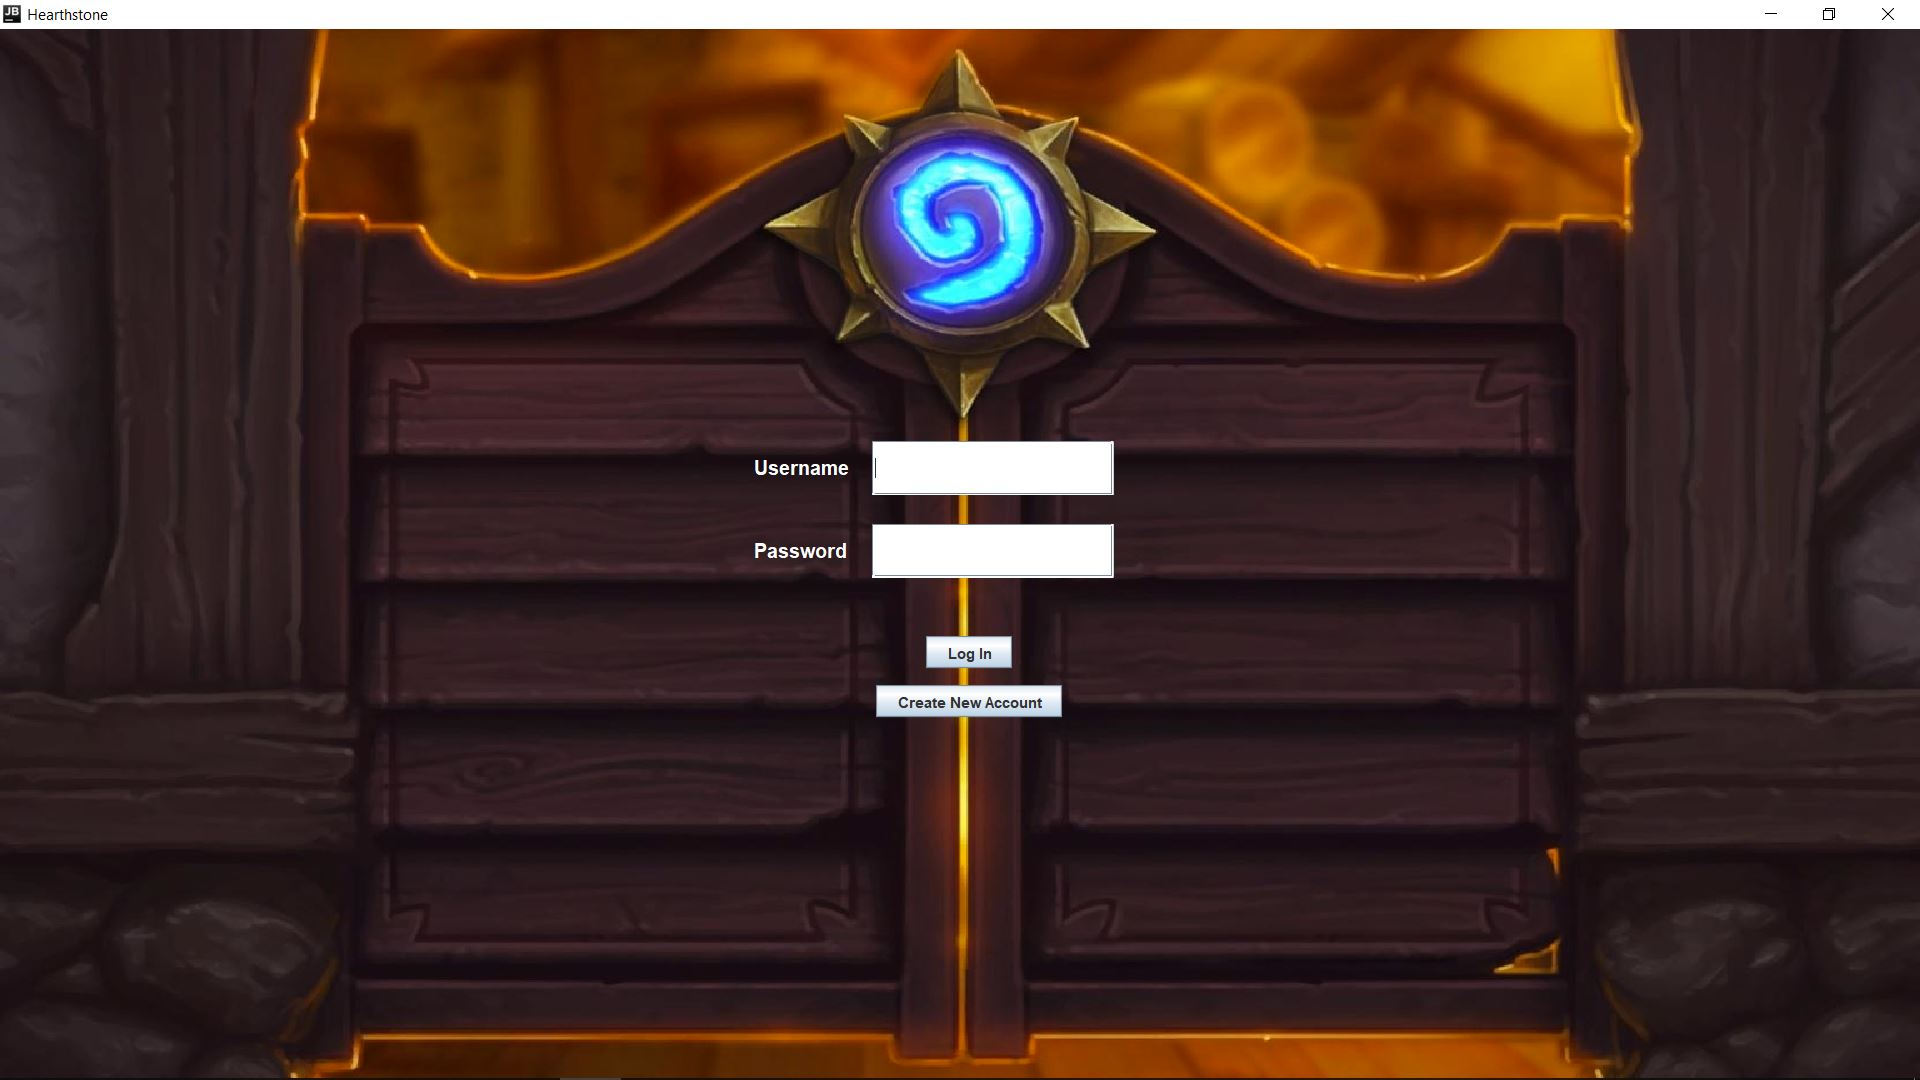
\includegraphics[scale=0.4]{loginPanel.JPG}
	\caption{The login panel}
	\label{loginPanel}
\end{figure}

\subsection{\texttt{MainMenuPanel}}
This panel is responsible for the main menu of the game, which leads the user to collections, store, status, or playground. It consists of a background and simple buttons as depicted in figure \ref{mainmenu}.
\begin{figure}[h!]
	\centering
	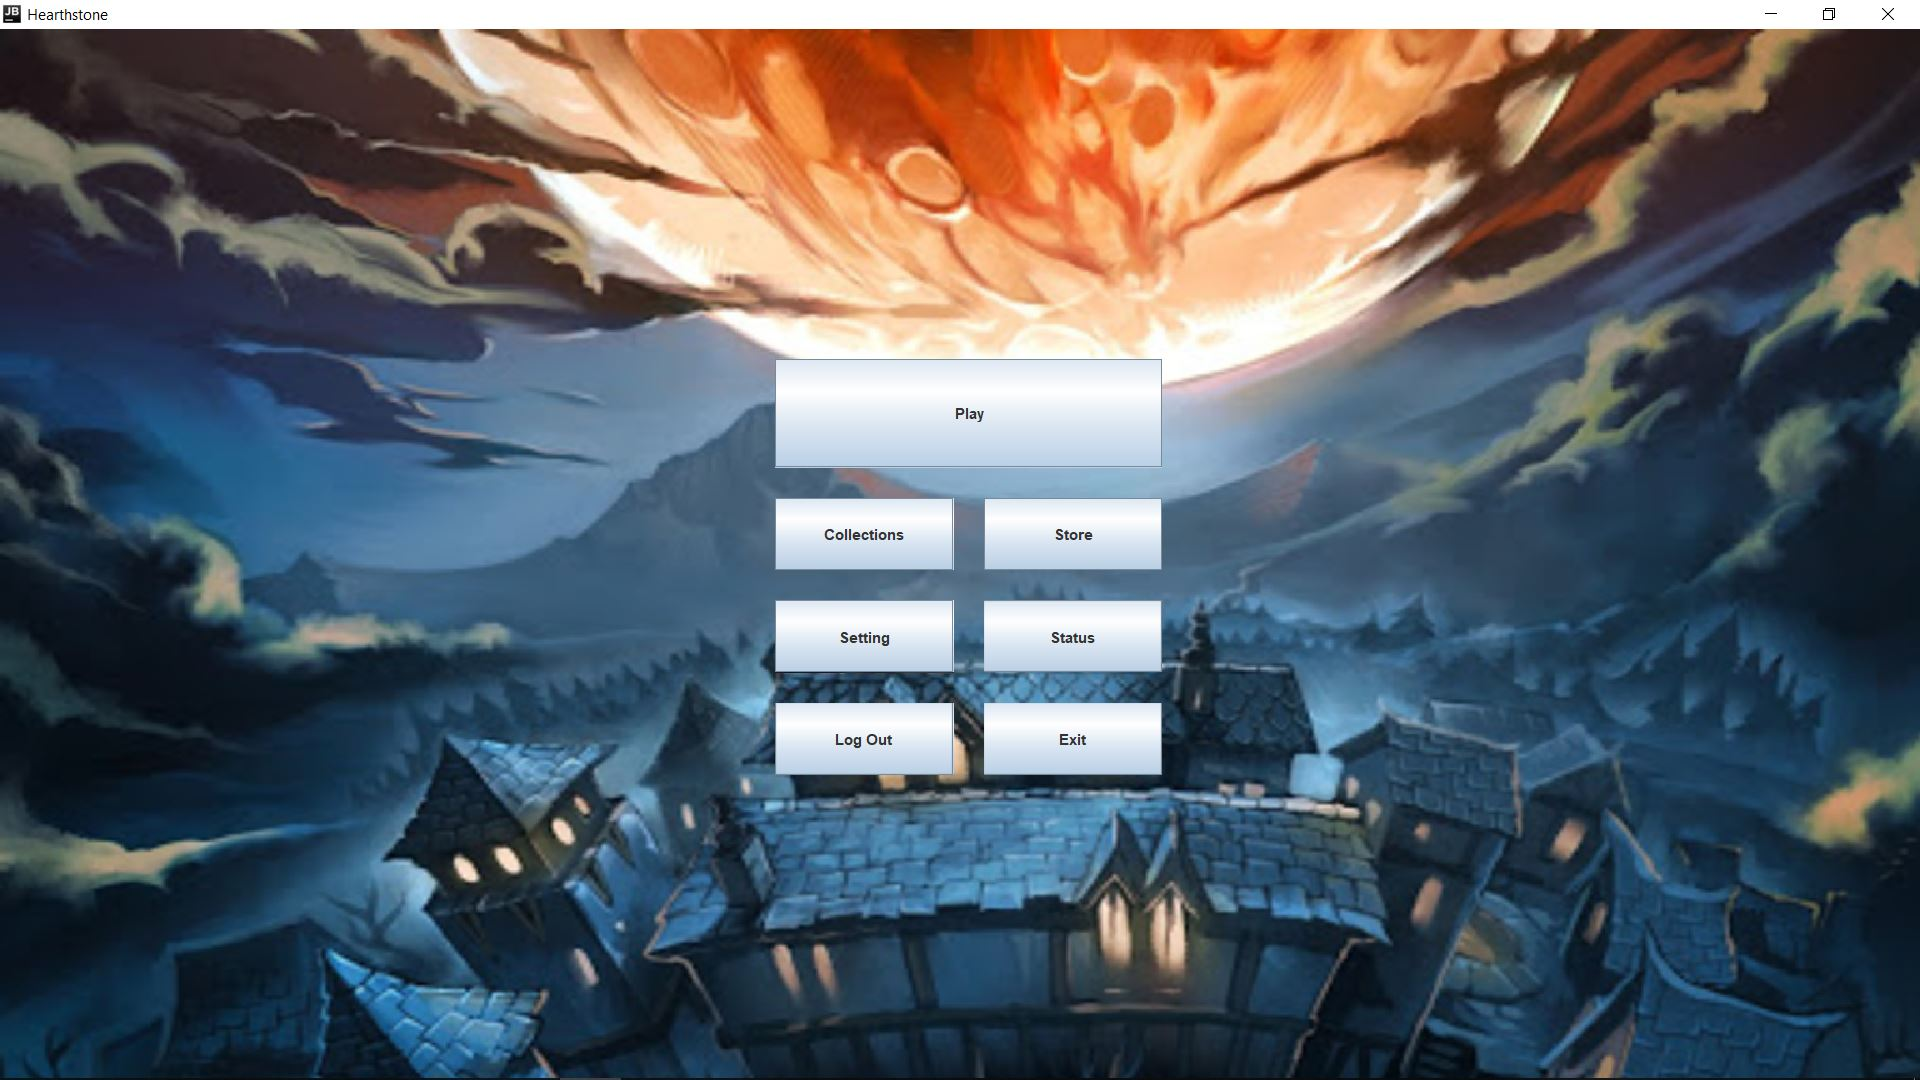
\includegraphics[scale=0.4]{mainmenuPanel.JPG}
	\caption{The main menu panel}
	\label{mainmenu}
\end{figure}

\subsection{\texttt{CollectionsPanel}}
This panel is the graphical implementation of the games collections. It consists of some smaller panels, some responsible for holding different button, and one responsible for showing cards. Each card is actually a \texttt{JButton} with a background, so one can easily click on them to directly buy or sell a card. On the panel on the right of collections, a \texttt{CardLayout } layout manager has been used to have two cards, one for a list of decks and another to show the cards present in each deck. These two are shown in figures  \ref{cl1} and \ref{cl2} respectively.

\begin{figure}[h!]
	\centering
	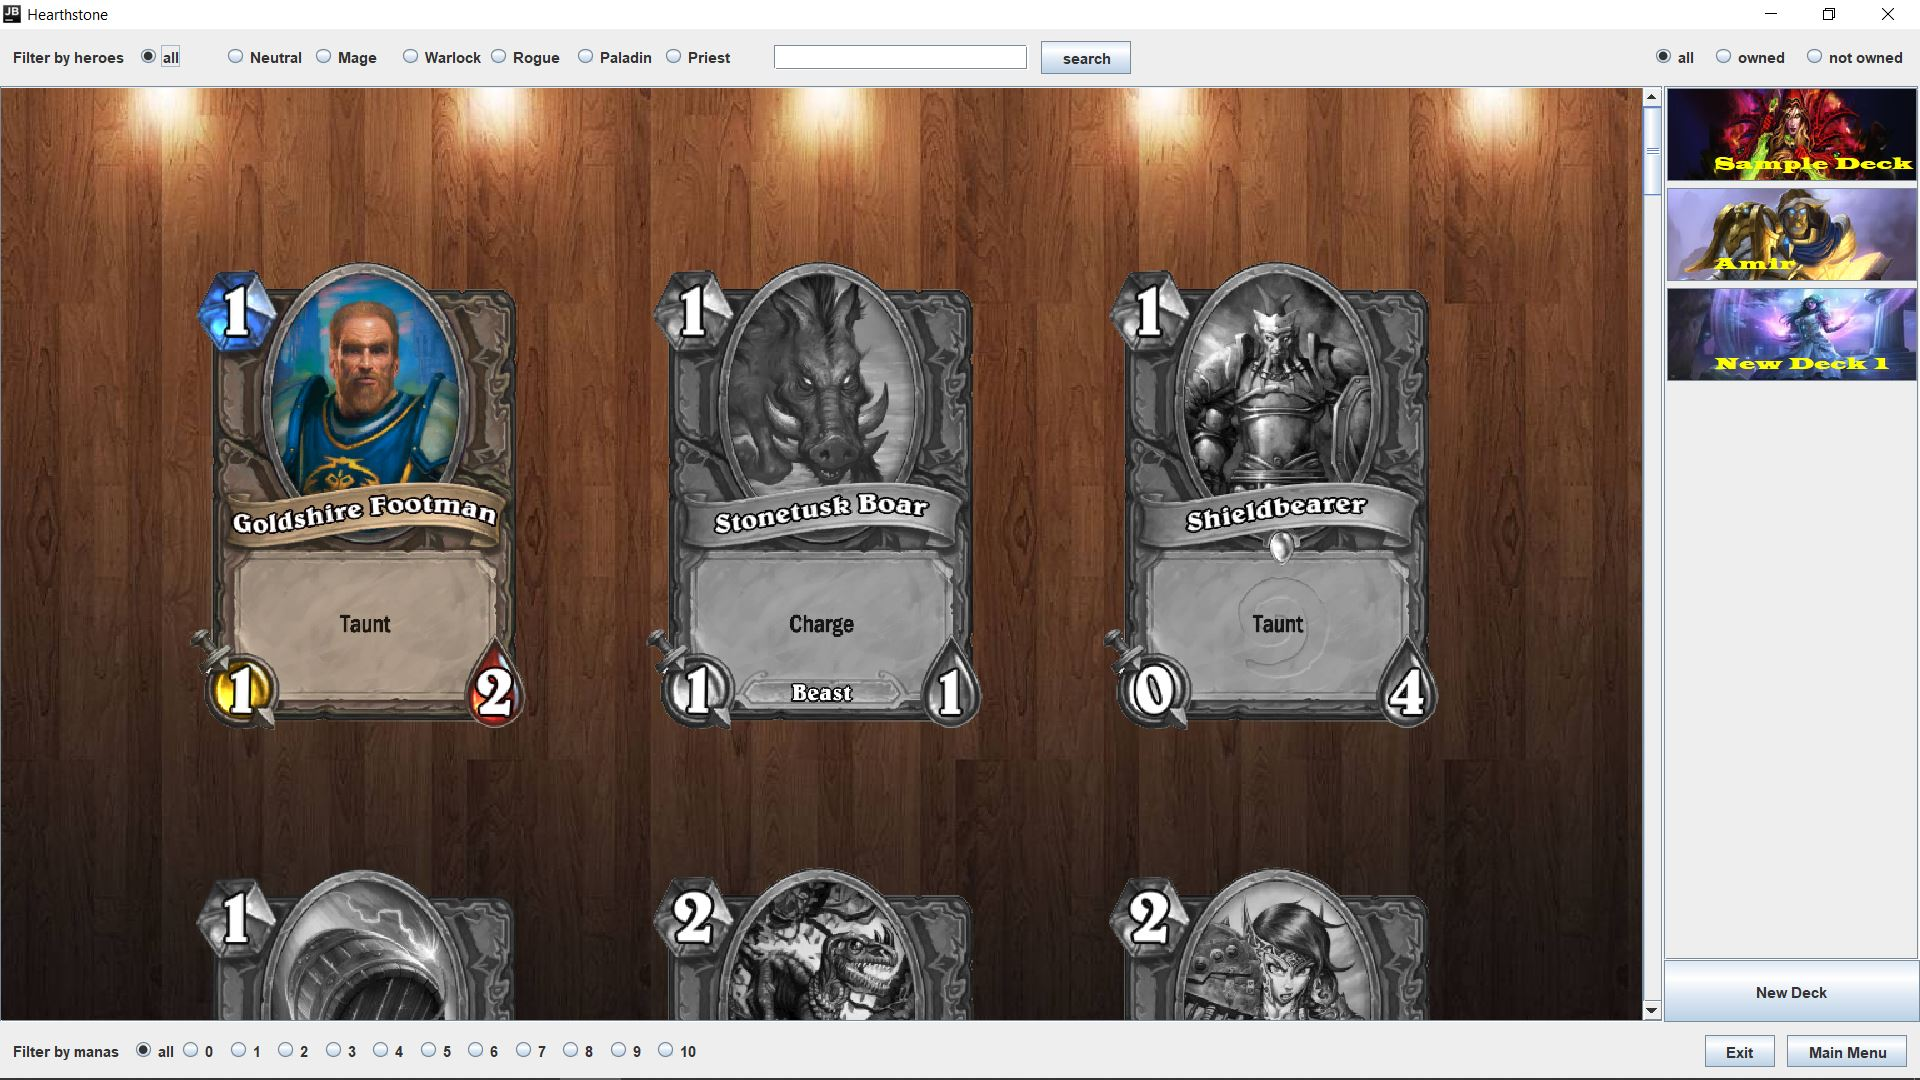
\includegraphics[scale=0.4]{collectionPanel1.JPG}
	\caption{The collections panel and the list of decks}
	\label{cl1}
\end{figure}

\begin{figure}[h!]
	\centering
	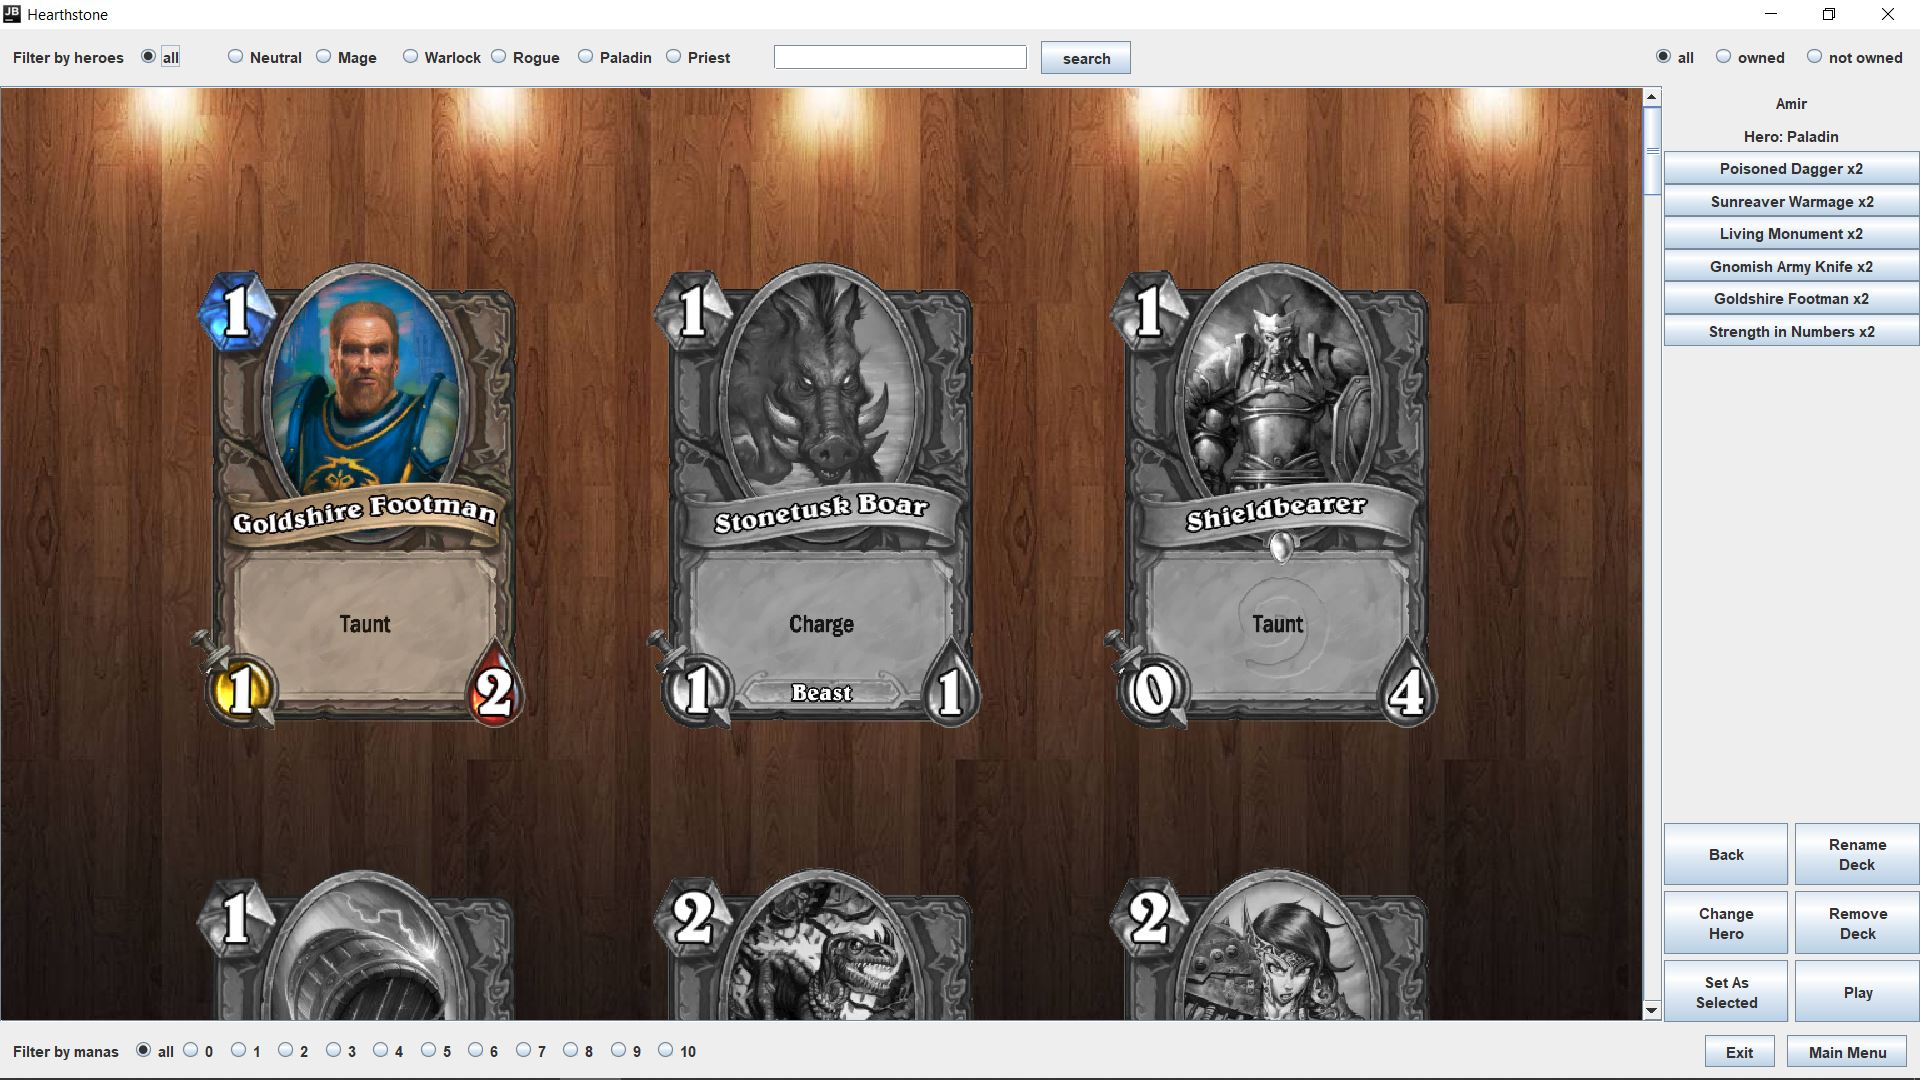
\includegraphics[scale=0.4]{collectionPanel2.JPG}
	\caption{The collections panel and the cards of a deck}
	\label{cl2}
\end{figure}

\subsection{\texttt{StorePanel}}
This panel, as depicted in figure   \ref{store}, is very similar to the collections panel and the implementation is quite the same. Actually the collections panel almost contains an independent store within itself, so one can easily design a store panel after having one for the collections.

\begin{figure}[h!]
	\centering
	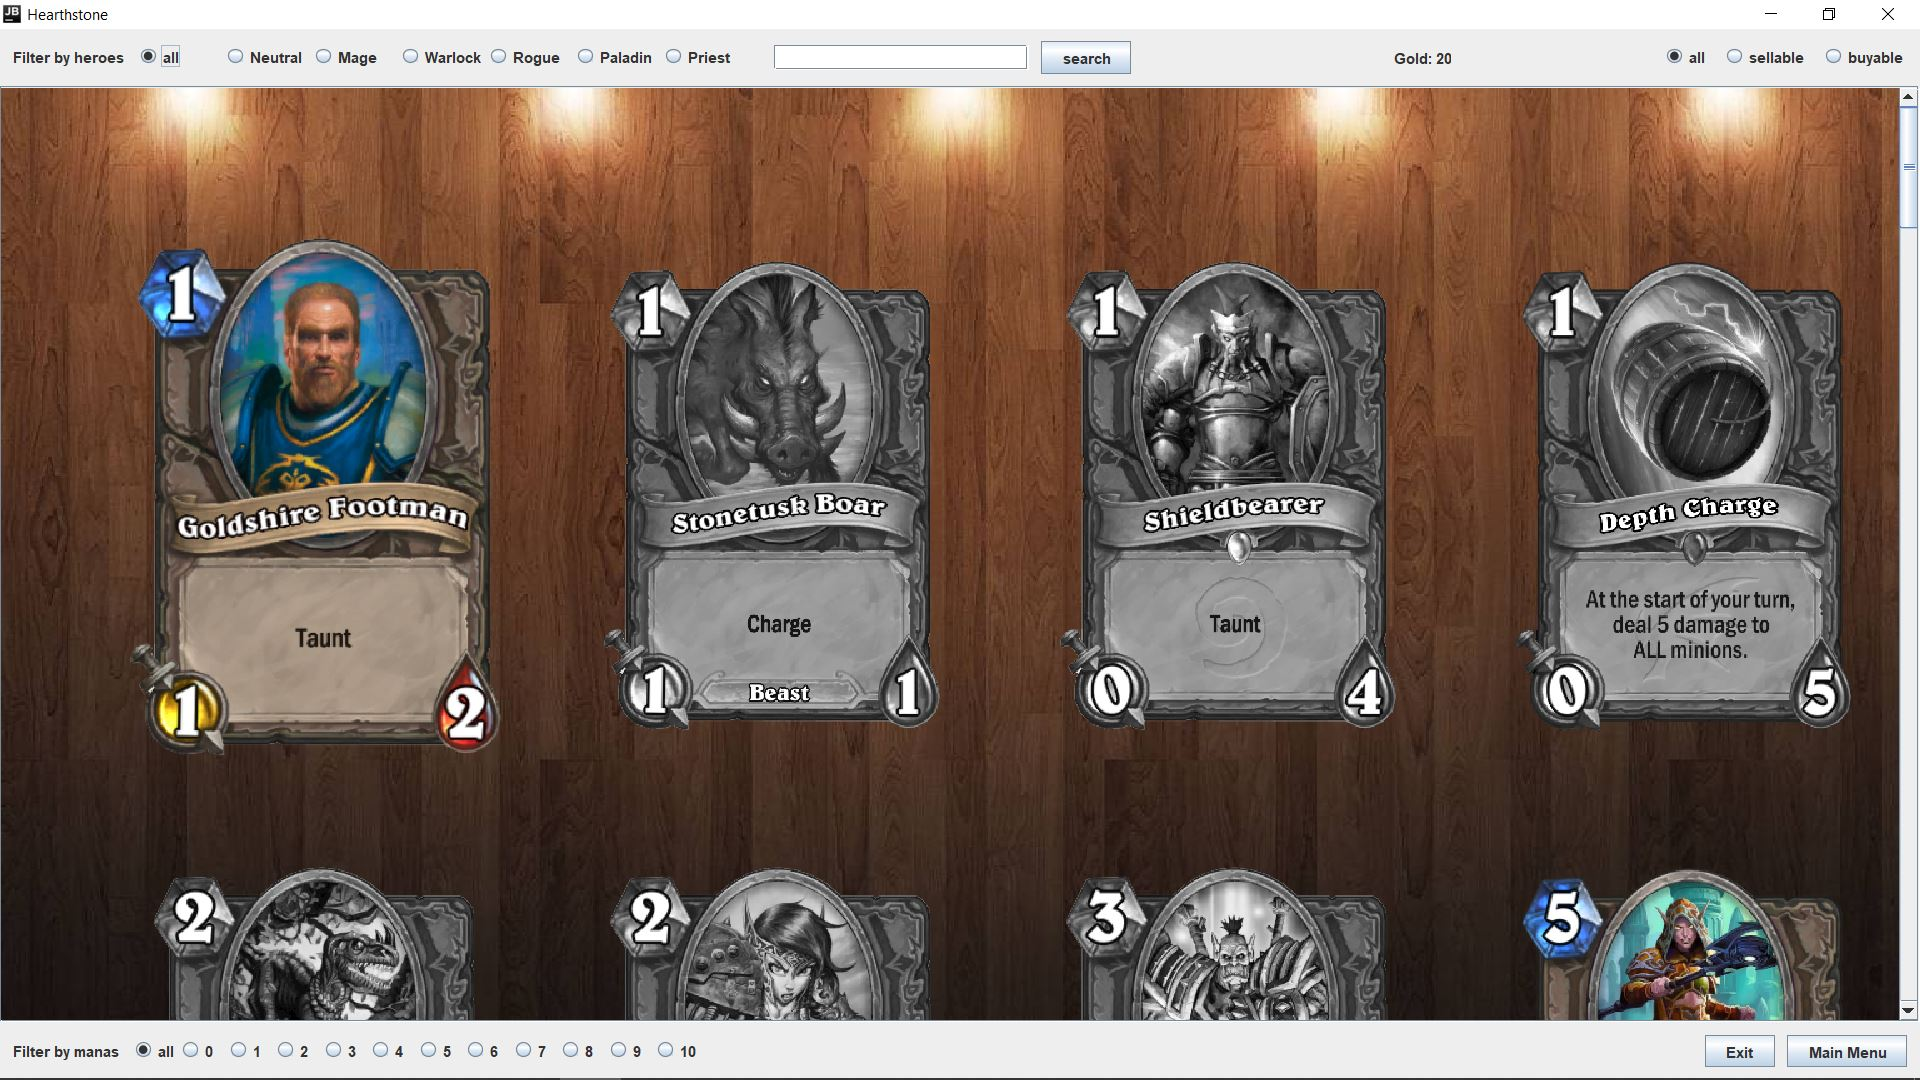
\includegraphics[scale=0.4]{StorePanel.JPG}
	\caption{The store panel}
	\label{store}
\end{figure}

\subsection{\texttt{StatusPanel}}
This panel has also inherited most of its graphical features from the collections panel (by inheritance, we mean the similarity in appearance not the popular concept of programming). It includes two separate panels, one for showing the statistics (the larger panel on the left), and another to show a list of decks or the cards inside a deck. This is shown in figures  \ref{stat1}  and \ref{stat2}.
\begin{figure}[h!]
	\centering
	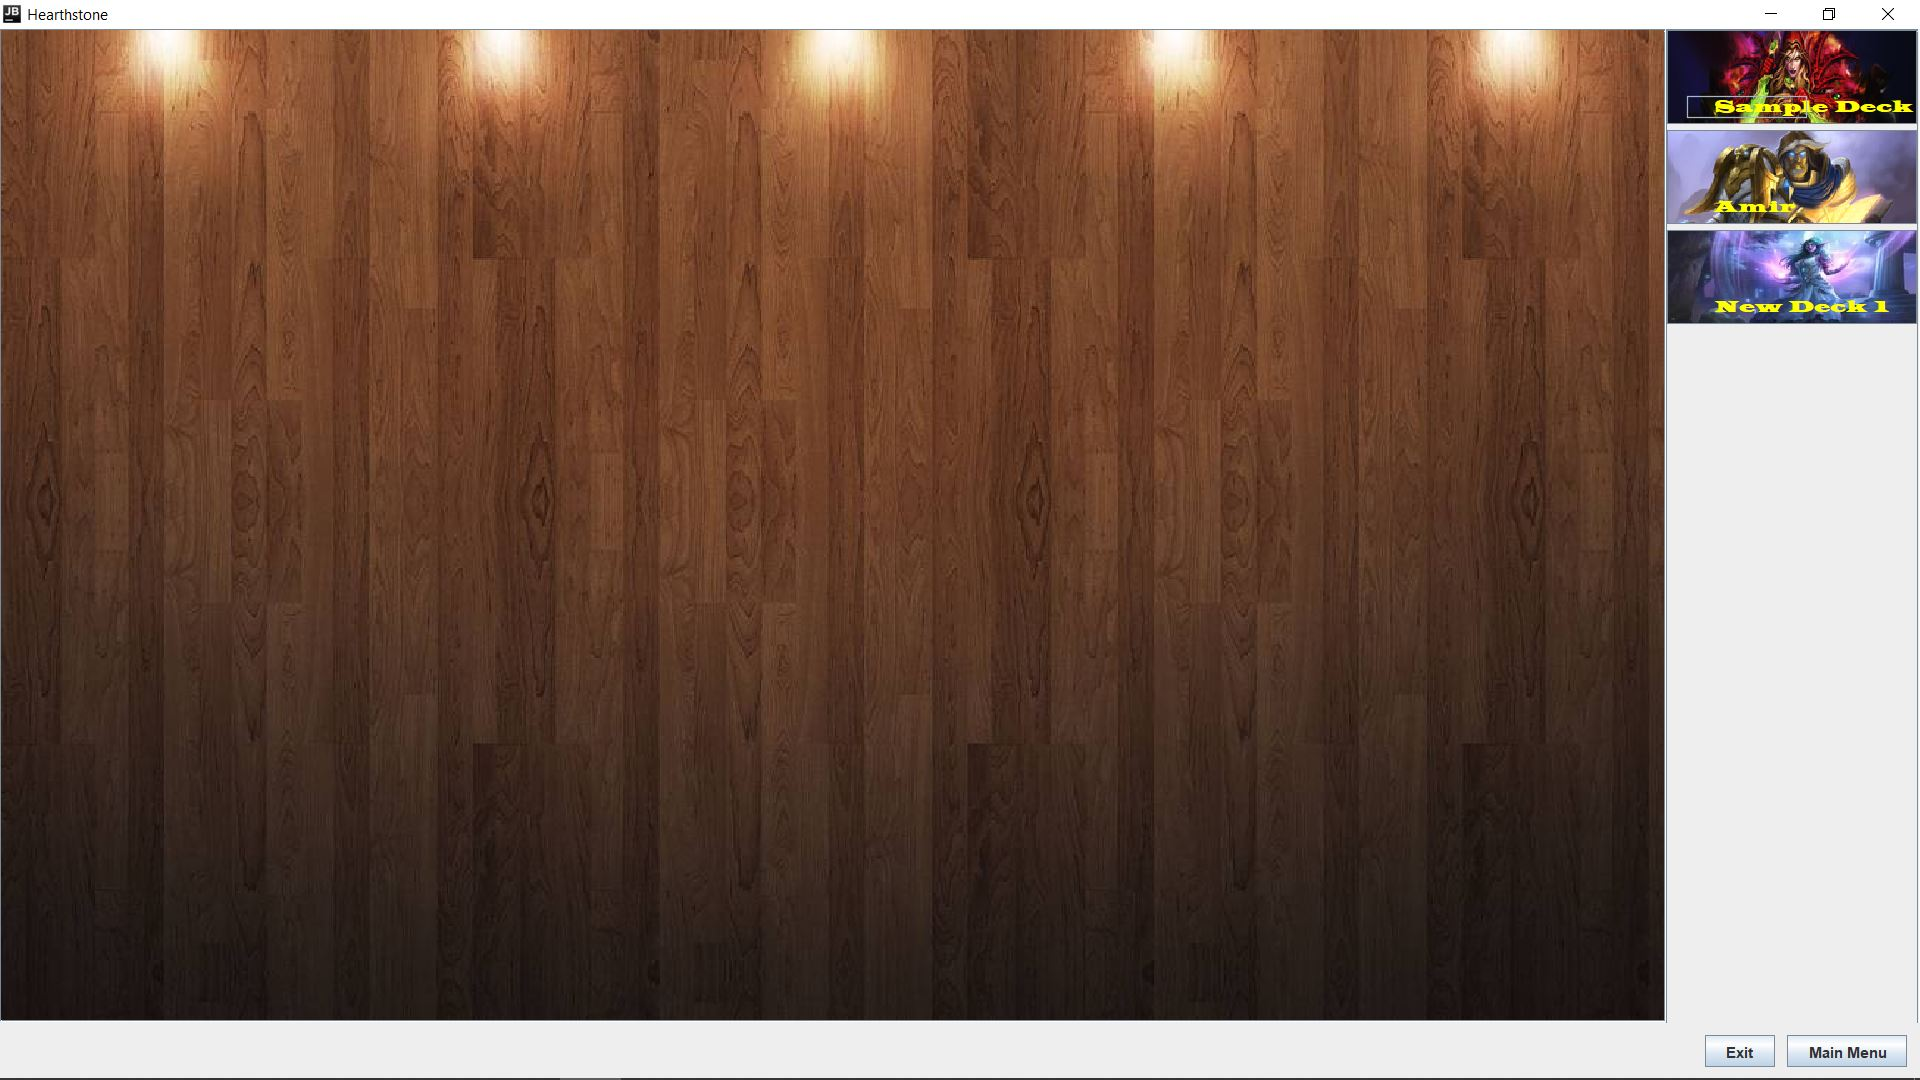
\includegraphics[scale=0.4]{statusPanel1.JPG}
	\caption{The status panel with no decks selected}
	\label{stat1}
\end{figure}

\begin{figure}[h!]
	\centering
	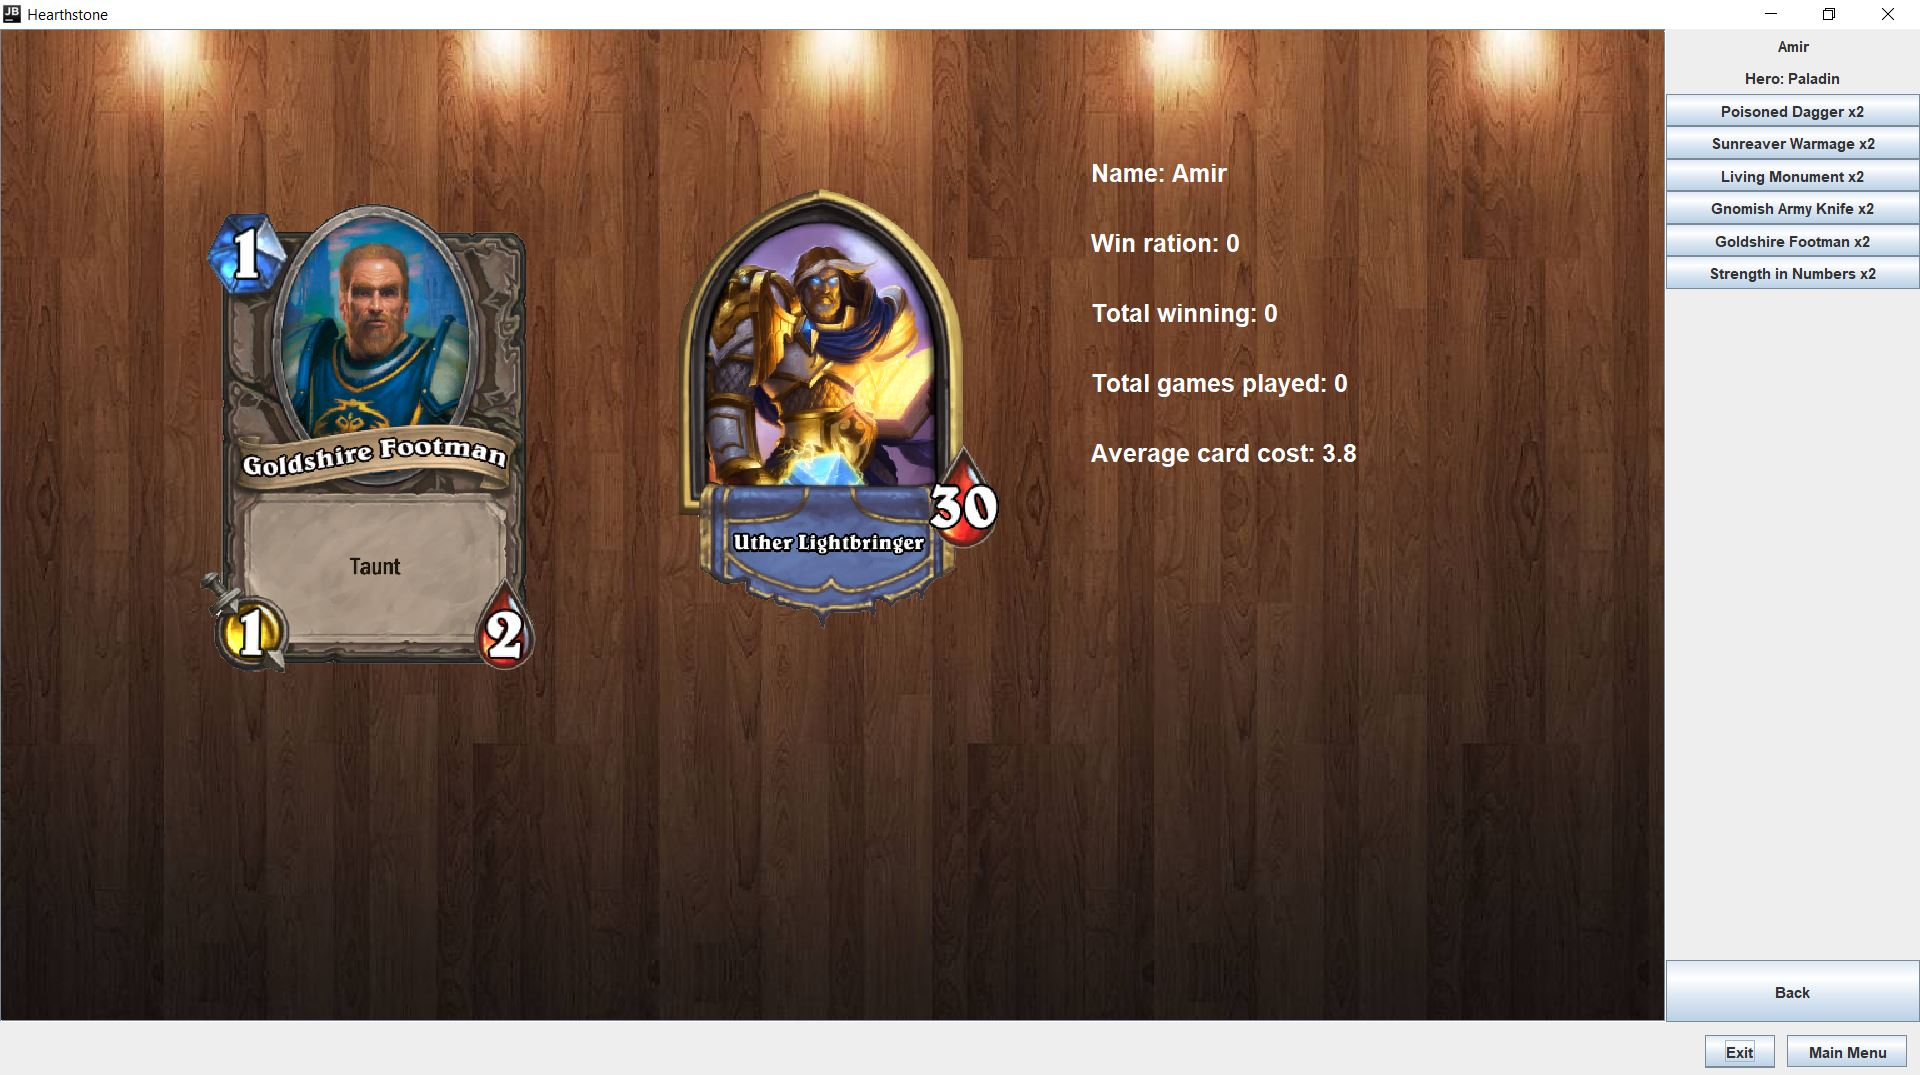
\includegraphics[scale=0.4]{statusPanel2.JPG}
	\caption{The status panel with a selected deck}
	\label{stat2}
\end{figure}

\subsection{\texttt{PlayPanel}}
This is the panel on which the actual game takes place. We have used the absolute positioning system on this panel, since we need to organize the objects neatly on the background picture. Also for each card we have used a panel, so we can recognize clicks, mouse enters, and mouse exits; and moreover, it is an easy element to work with. The result is depicted in figure \ref{playPanel}.
\begin{figure}[h!]
	\centering
	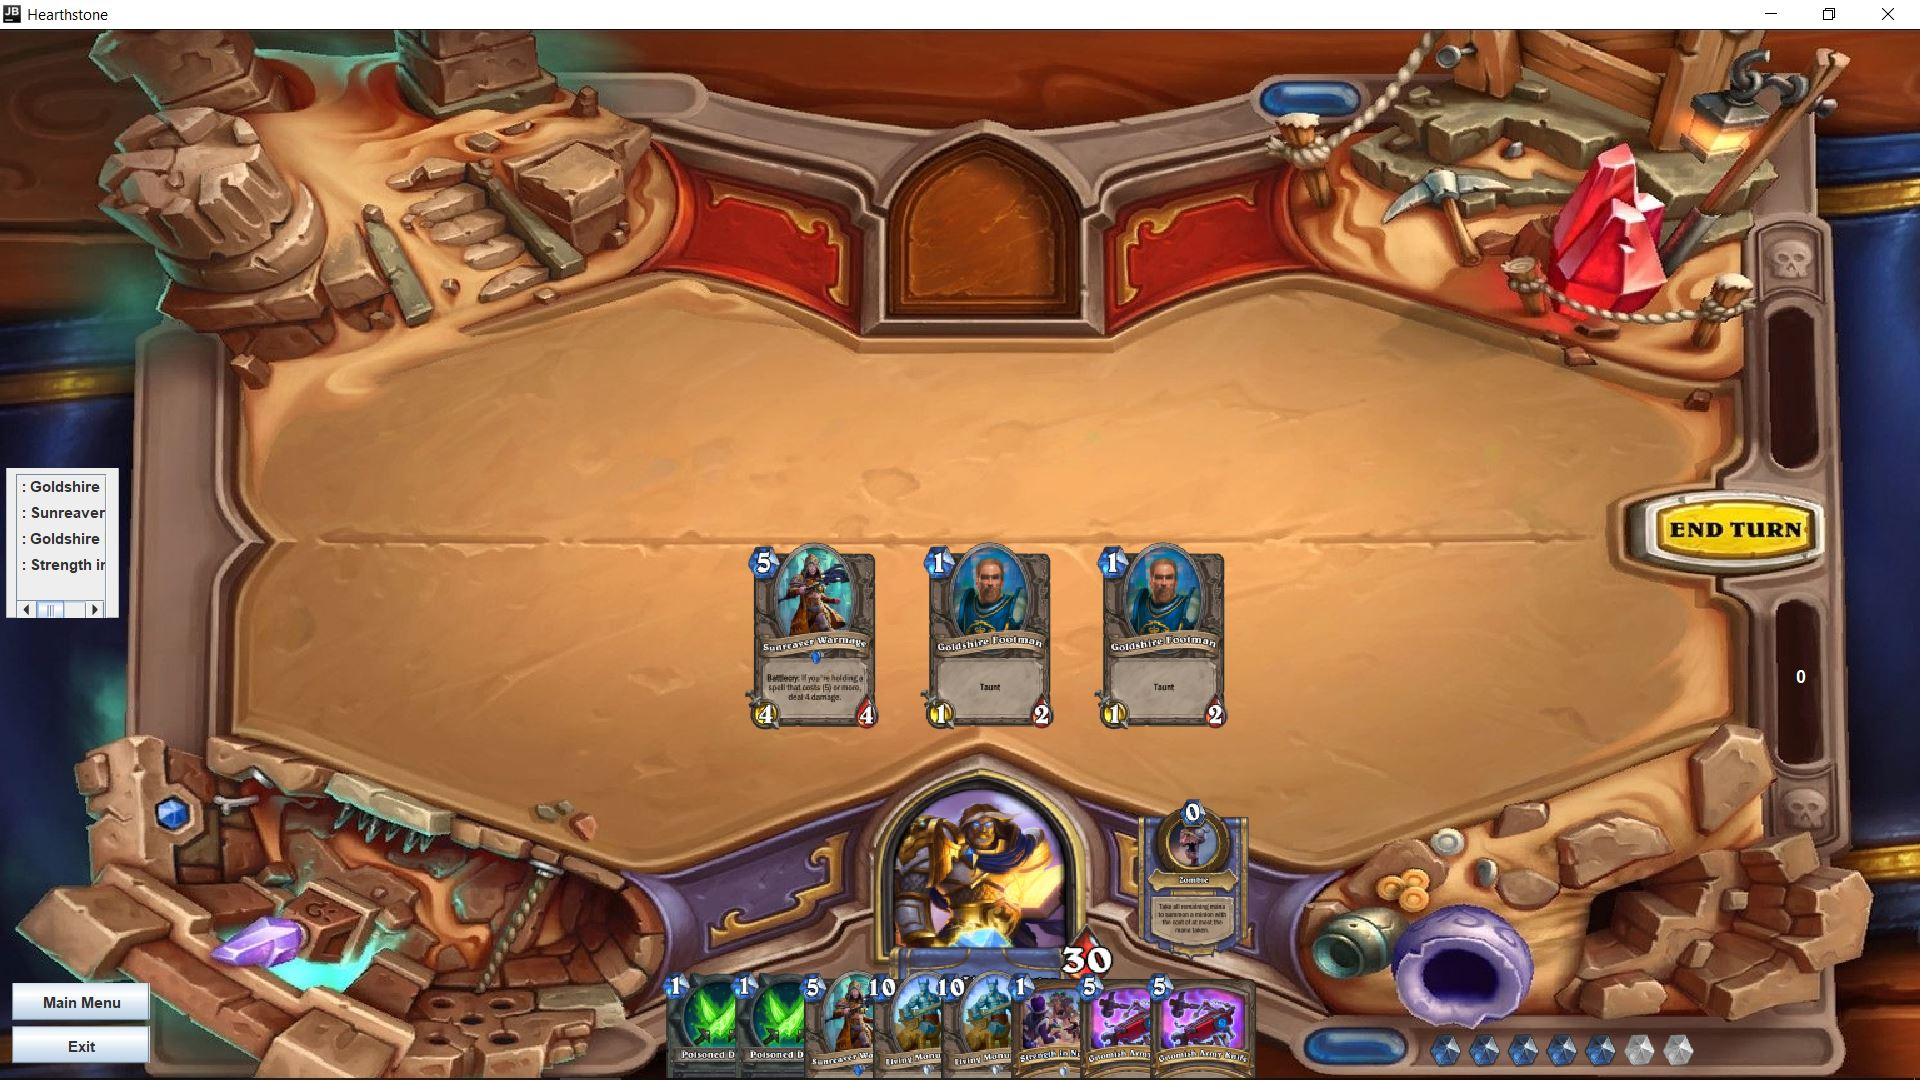
\includegraphics[scale=0.4]{playPanel.JPG}
	\caption{The battlefield of the game}
	\label{playPanel}
\end{figure}

\clearpage
\section{Packages \texttt{Events} and \texttt{Listeners}}
The concepts of \textit{events} and \textit{event--listeners} are of great importance in our program design. Using events and listeners, we can model the occurrence of an event and the jobs other modules should do after that. We have designed many event classes (all extending \texttt{EventObject}) and many listeners (all extending \texttt{EventListener}) although we could have done without them, or at least without most of them. Many of these classes have the same code within themselves, but the reason we created them separately is to make the structure of our design more easily understood. Most of these events happen when a button is pressed, and the listener (which is set by the main frame) will run a method to do the proper job. This structure results in the GUI being almost unaware of what goes on in the game logic, which was initially one of our main design interests.

\clearpage
\section{Packages \texttt{Dialogs} and \texttt{Utils}}
Apart from the main panels, we sometimes need other graphical utilities. This is why we have designed two more packages. The package \texttt{Dialogs} consists of different classes which produce a new small frame to get a response from the user (or to simply deliver a message). Needing them for simple message delivery, getting a yes--no response, getting a multiple choice response, or a text input; we have designed four dialog classes.\\

The package \texttt{Utils} also includes some extensions of standard classes, which could be useful in our program. The class \texttt{BackgroundedPanel} extends \texttt{JPanel} and creates a panel with a background image. The class \texttt{backgroundJViewport} extends the class \texttt{JViewport} to implement a structure to have a panel with scroll bar and background image. Finally, the class \texttt{DynamicIcon} is used to create a \texttt{JButton} which has an image icon and a text written over it.

\clearpage
\section{Resources}
In this section, we introduce all external resources we have used for this phase of the project.
\subsection{The Code}
Most of the code is generated by the author without external help (other than some normal internet searches). The only part to be mentioned specifically is the class \texttt{ImageLoader} from the package \texttt{Utilities}, which has been initially taken from the asteroid project provided by the course instructors.

\subsection{Game Photos}
This project includes many pictures for the GUI. These pictures have either been downloaded directly, or designed by the author. The first group have mostly been downloaded from \url{https://hearthstone.gamepedia.com/Hearthstone_Wiki}. For the cards which we needed to design, we have used \url{http://www.hearthcards.net/}, a website that lets you design any card with an incredibly efficient interface.









\end{document}






